\chapter{Model Architecture}

In this chapter, the architectures of several models are presented. Section \ref{modpoly} gives a comprehensive explanation to the structure of PolygonRNN, while section \ref{modfpn} looks into the FPN part of Mask R-CNN. Considering our problem, we combine PolygonRNN and FPN part of Mask R-CNN together and come up with a new model, which is called \modelnameshort\ (\modelnamelong, see section \ref{modmer}). In theory, the proposed model can find out the bounding boxes of buildings within an aerial image and give geometrical shape for each building.
 
\section{PolygonRNN}\label{modpoly}

PolygonRNN is the core model for finding geometrical shapes in this project. Figure \ref{fig:simppoly} shows the simplified structure of PolygonRNN. The CNN part (see subsection \ref{modcnn}) can capture image features through multilayer convolutions and max pooling, which is then fed into the RNN part (see subsection \ref{modrnn}), which can sequentially predict spatial location of the new vertex with the highest probability at each time step.

\begin{figure}[!h]
	\centering
	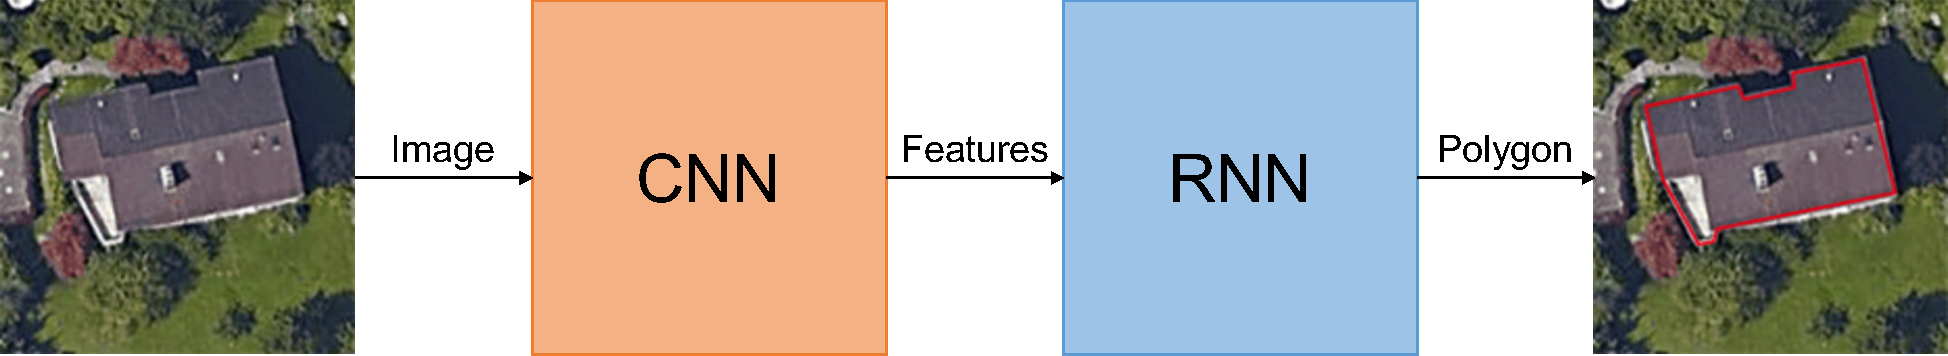
\includegraphics[width=\fig\textwidth]{3-00.pdf}
    \caption[The simplified model architecture of PolygonRNN]{The simplified model architecture of PolygonRNN.}
    \label{fig:simppoly}
\end{figure}

\subsection{CNN Part}\label{modcnn}

The CNN part of PolygonRNN uses VGG-16. Actually, VGG-16 is a form of VGGNet, which is very structured and focusing on deepening the  neural network without a large number of parameters. It generally believes that deeper networks have stronger expressive capabilities than shallow networks, and can accomplish more complex tasks. It also proven in practice that VGGNet has made great progress in performance compared to its previous network architecture (e.g. AlexNet).

The `16' in VGG-16 means that it is a VGGNet with 16 layers containing parameters (13 convolutional layers and 3 fully connected layers). It has around 138 million parameters in total. Figure \ref{fig:vgg16} shows its detailed network structure. From the figure we can see that VGG-16 continuously does convolution with $3\times3$ small kernels and makes $2\times2$ max pooling. As the network deepens, the width and height of the image are reduced by half after each max pooling, and the number of channels is also doubly increasing after some convolution.

\begin{figure}[!h]
	\centering
	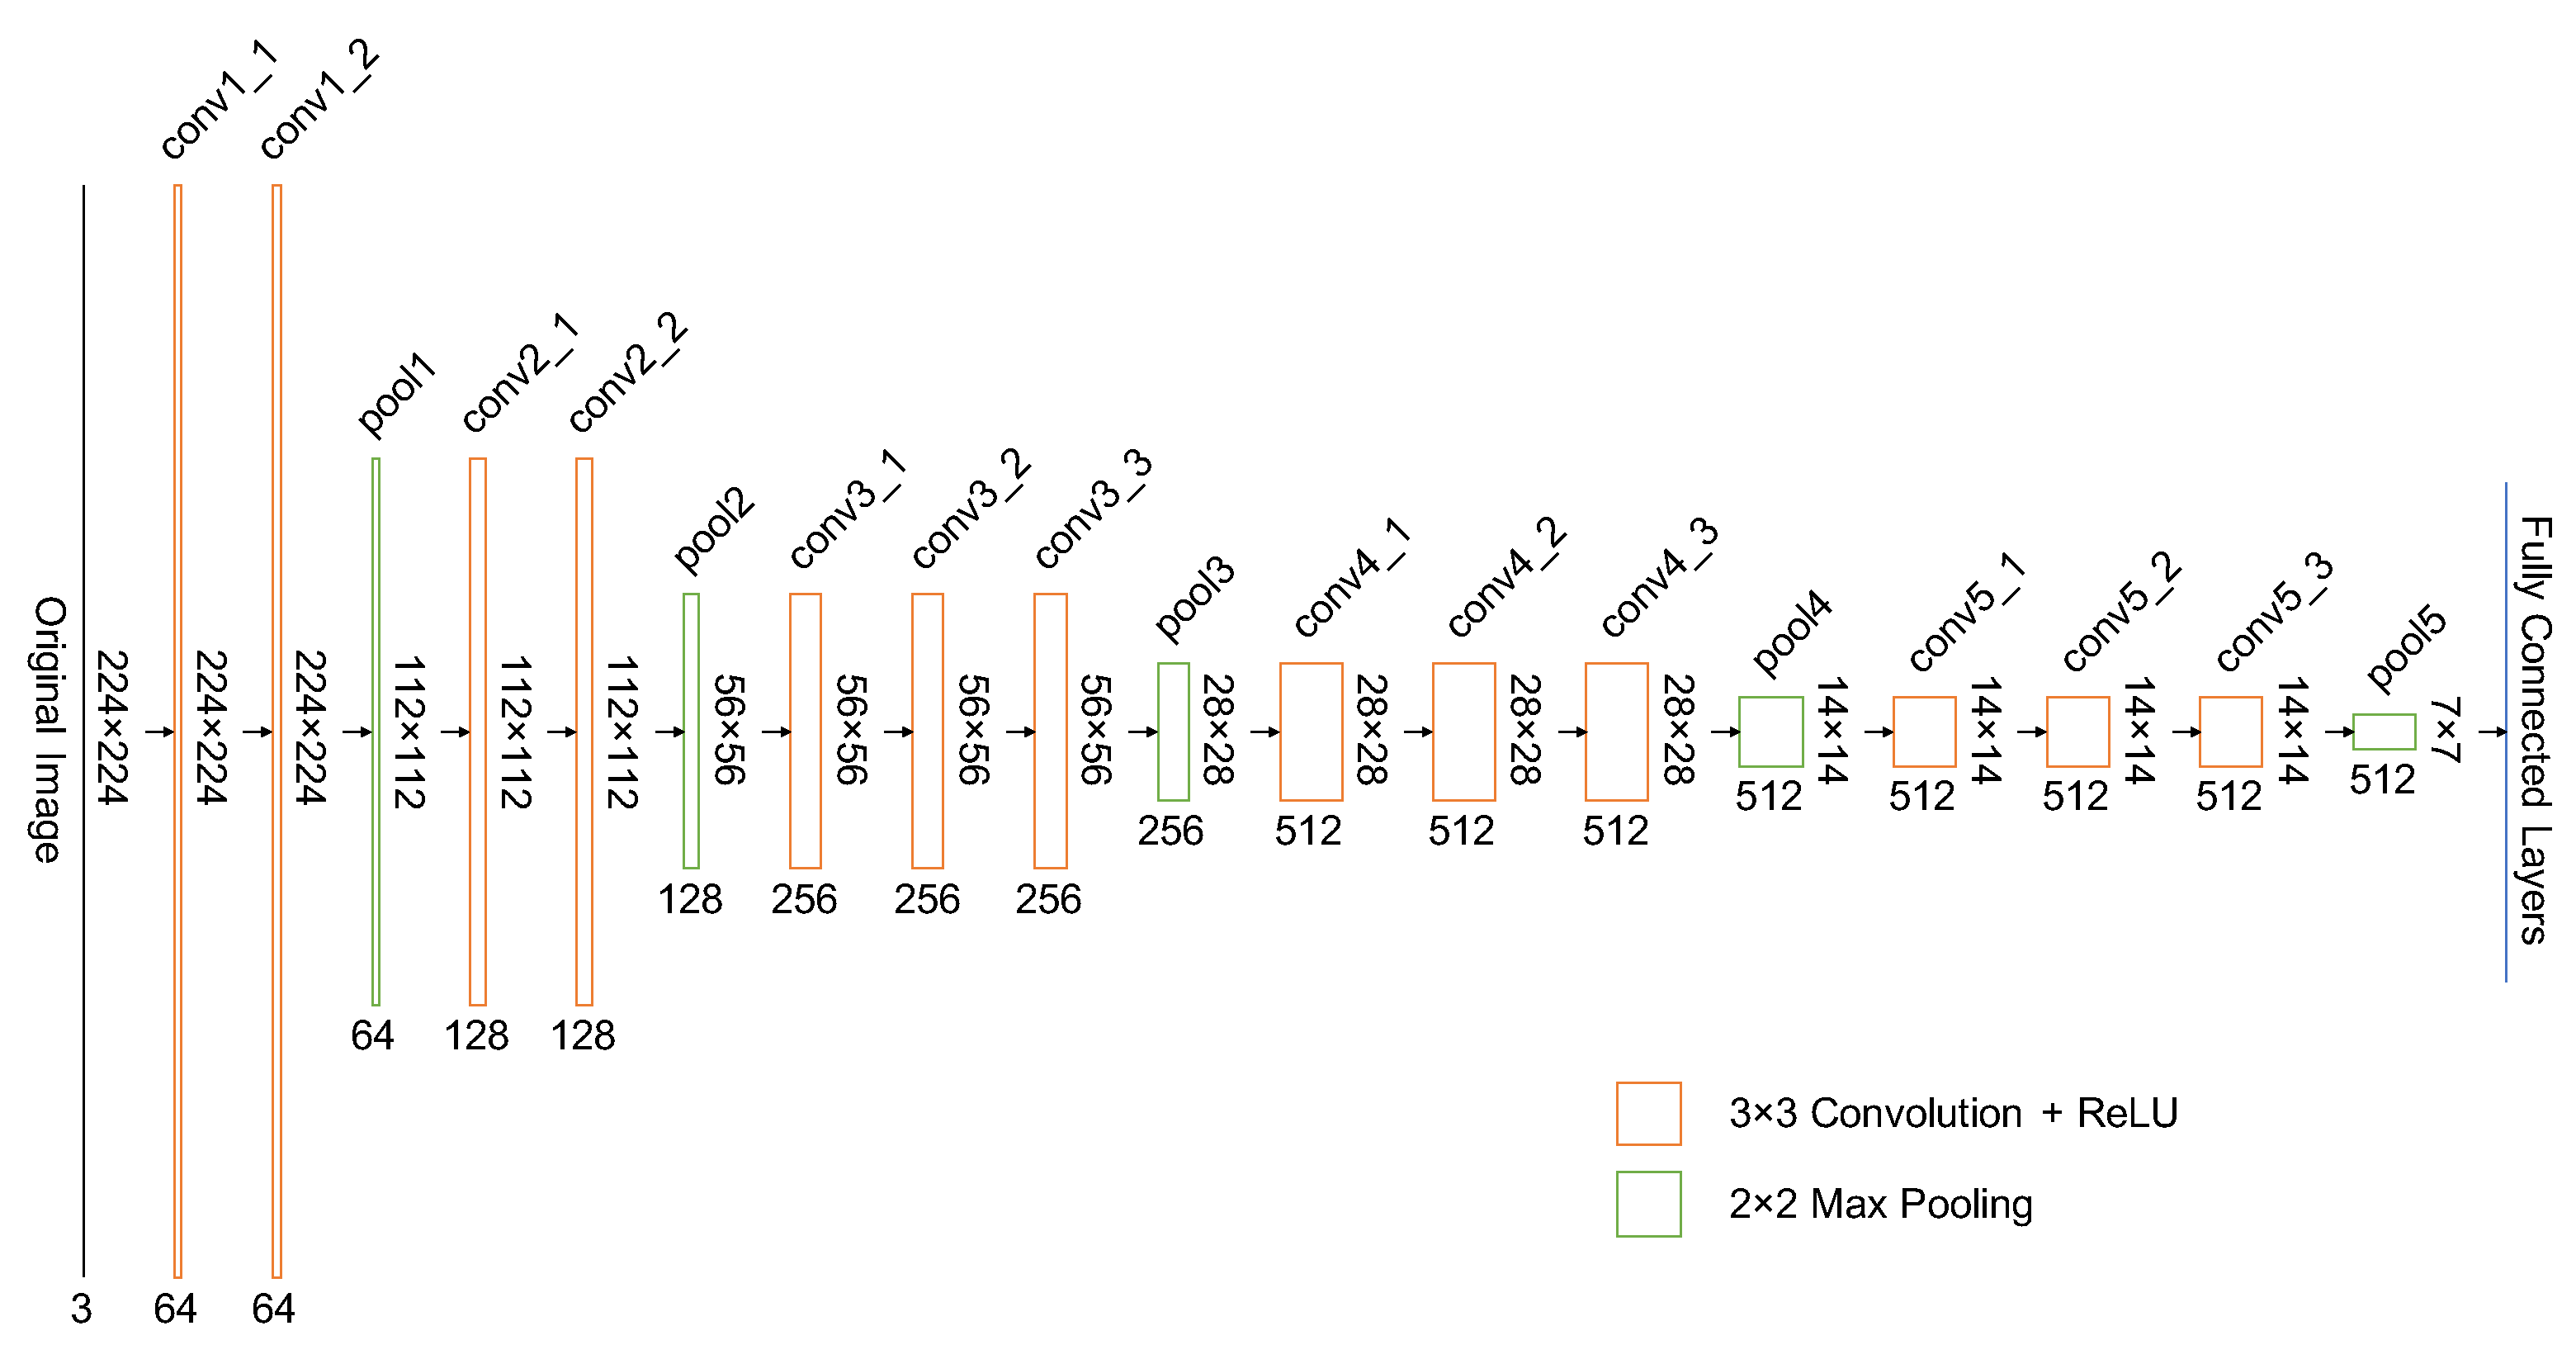
\includegraphics[width=\fig\textwidth]{3-01.pdf}
    \caption[VGG-16 architecture]{VGG-16 architecture. Only convolutional layers and maximum pooling layers are presented.}
    \label{fig:vgg16}
\end{figure}

VGG-16 was mostly used for image classification before, so after the convolutional layers and max pooling layers there are fully connected layers and softmax layer for the class labels. However, these two kinds of layers are not required for VGG-16 used in PolygonRNN, because the CNN here is working as a feature extractor and mask predictor. Layer \lstinline{pool5} is omitted as well because of the too low resolution.

\paragraph{Feature Extraction} The modified VGG-16 provides RNN with useful features, which are taken from different convolutional and max pooling layers. Specifically, the features are extracted from layer \lstinline{pool2}, \lstinline{pool3}, \lstinline{conv4_3} and \lstinline{conv5_3}. Note that since the resolution of final features is fixed, when taking features from layer \lstinline{pool2} and \lstinline{conv5_3}, it requires another max pooling and upsampling respectively. All of these can be seen in figure \ref{fig:mdfvgg16}.

\begin{figure}[!h]
	\centering
	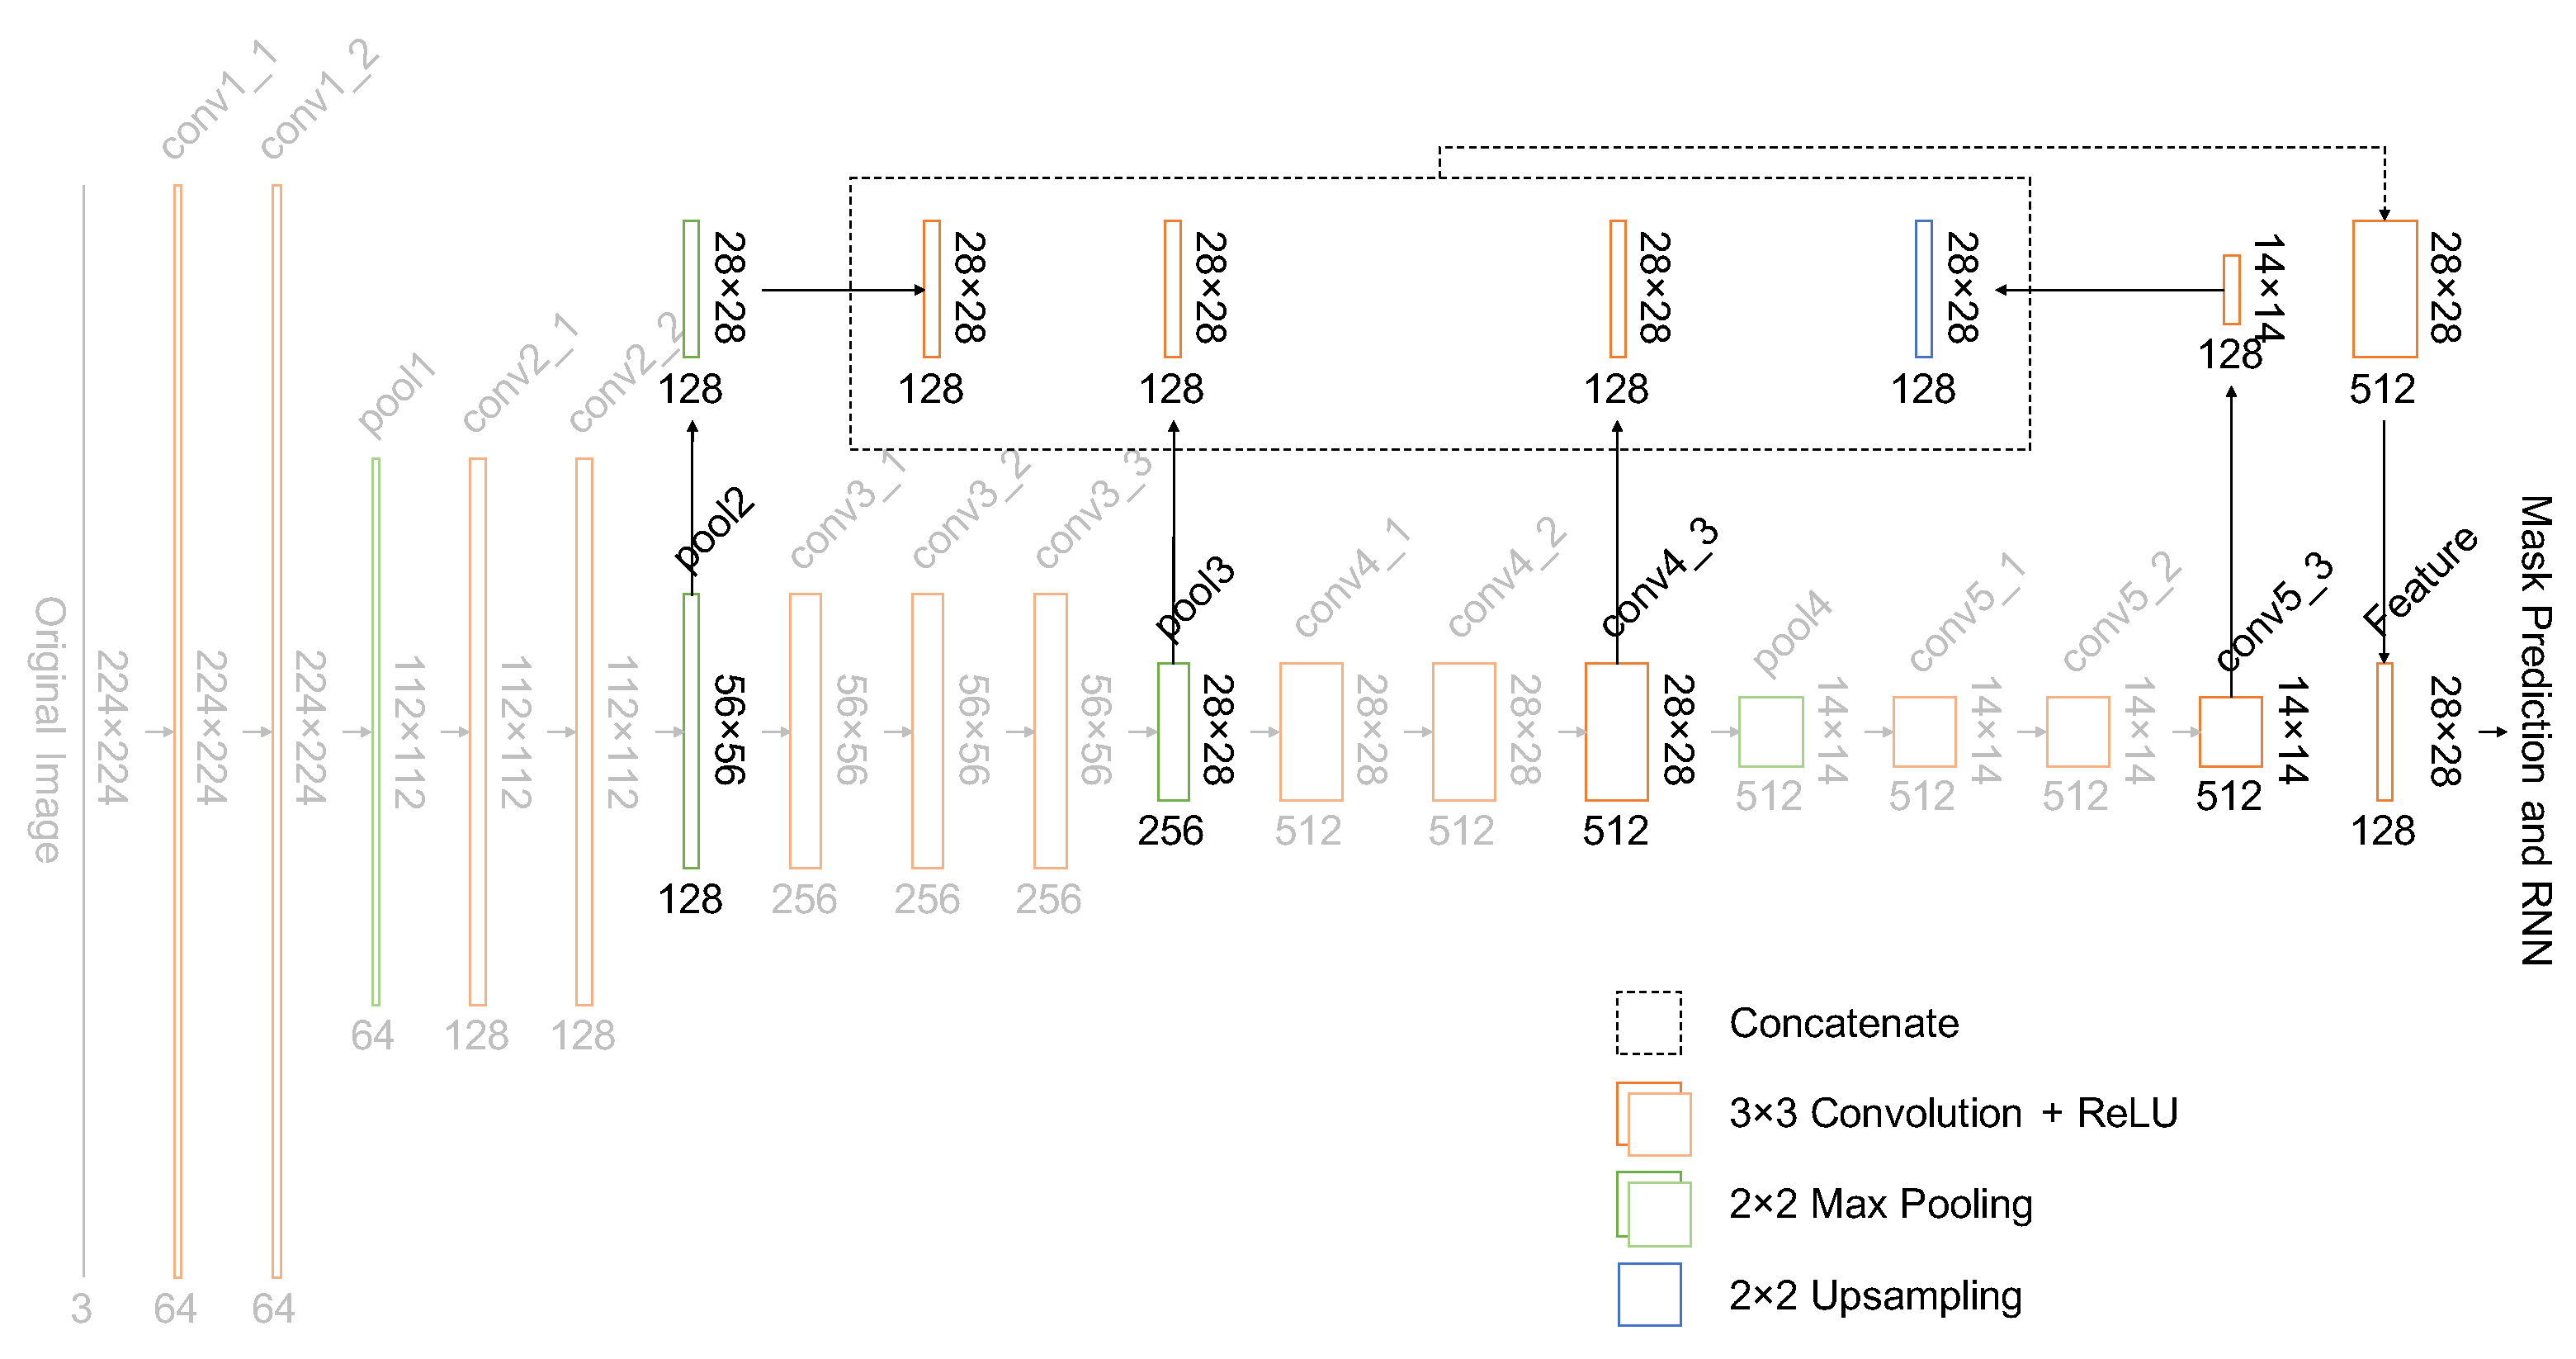
\includegraphics[width=\fig\textwidth]{3-02.pdf}
    \caption{Modified VGG-16 architecture in PolygonRNN.}
    \label{fig:mdfvgg16}
\end{figure}

\paragraph{Mask Prediction}
Another function of the CNN part is to predict masks of boundary and vertices in a low resolution (one eighth of the original). Figure \ref{fig:vgg16mask} shows the mask prediction phase. Different from the ReLU function used in the former convolutional layers, the activation function used here is the sigmoid function. Each entry of the boundary or the vertices mask indicates the probability that the pixel is located in the boundary or is a vertex respectively. The features and two masks are then sent into RNN together.
\begin{figure}[!h]
	\centering
	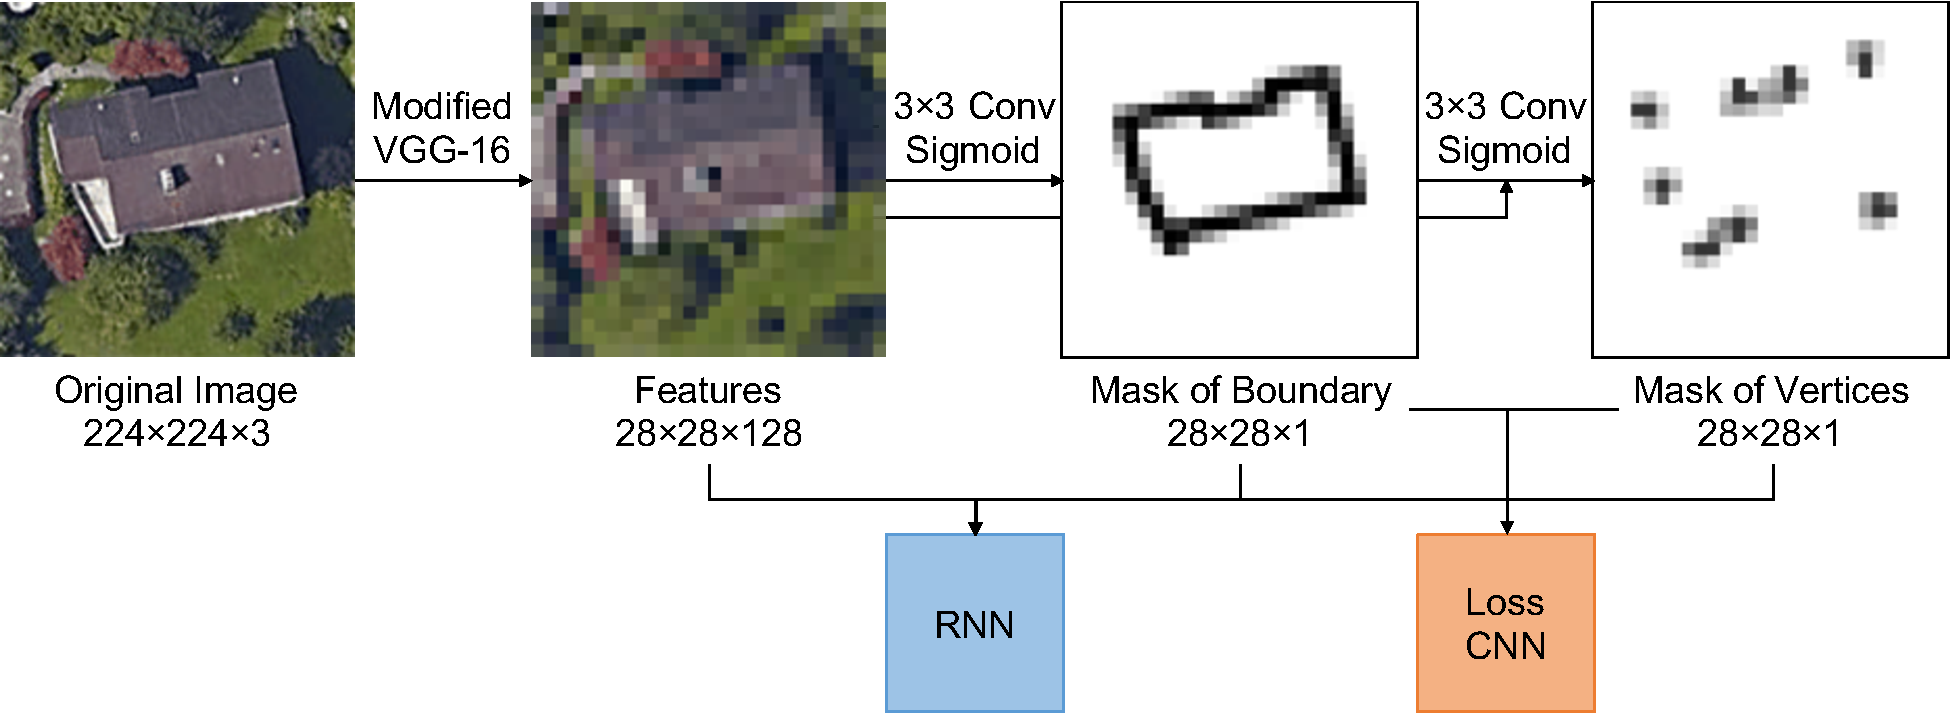
\includegraphics[width=\fig\textwidth]{3-03.pdf}
    \caption[Mask prediction of VGG-16]{Mask prediction of VGG-16. Note that the mask of vertices is obtained by the convolution on the concatenation of the features and the mask of boundary.}
    \label{fig:vgg16mask}
\end{figure}

\subsection{RNN Part}\label{modrnn}
The model used for predicting polygon vertices is RNN. We have already mentioned in subsection \ref{relatpoly} that RNN is very powerful when data is related to time series, and in our case, we regards the polygon as a series of vertices.

We know that given two vertices on a polygon in an order (either clockwise or anticlockwise), the third vertex after the two points can be uniquely determined. What RNN here can do is to predict the probability distribution of the next vertex's position in a low resolution when given the history information about the two vertices before, as well as the image features and the position of the starting vertex. This process can be formulated as follows.
\begin{equation}\label{eq:vnext}
	p(v_t \mid v_{t-1}, v_{t-2}) = F(v_{t-1}, v_{t-2}, v_0, f), \forall t \in \{2,3,4,\ldots,T\},
\end{equation}
where $f$ denotes the extracted features by CNN (including the masks of boundary and vertices), $F(\cdot)$ denotes a function for computing the conditional probability, $T$ denotes the number of vertices of the polygon, $v_t$ denotes the vertex position at $t$-th prediction. Specifically, the vertex prediction problem can be formulated as a classification problem. The position of $v_t$ can be then quantized to the resolution of output grid, and we can thus use one-hot encoding for $v_t$'s representation.

\paragraph{End Signal} Note that the positions for $v_t$ are not only limited to the general output grid, the end signal for the closure detection of the polygon is also embedded in $v_t$, just like the `end of sequence' token \lstinline{<eos>} or \lstinline{</s>} in the RNN language model. Thus, the number possible assignments of $v_t$ equals to the resolution of the output grid plus one ($28\times28+1=785$ in our case). In order to correctly predict the end signal, the starting vertex $v_0$ is required for the conditional probability (equation \ref{eq:vnext}) calculation, as it tells the model when to finish the prediction phase. If the current prediction is the same as, or very close to the starting vertex $v_0$, $v_t$ will be forced to raise the end signal, indicating that the entire polygon is close, and the prediction phase is therefore complete. So generally, the end signal works when $t=T$.

\paragraph{Starting Vertex} In equation \ref{eq:vnext}, two special cases $p(v_0)$ and $p(v_1 \mid v_0)$ are not included yet. These two cases are different from the general case, and should be considered in addition. In particular, we can directly regard the mask of vertices (for example, the rightmost image in figure \ref{fig:vgg16mask}) predicted by the CNN as $v_0$'s unnormalized probability distribution $\tilde{p}(v_0)$, and choose the position with the highest probability for $v_0$'s assignment. As $v_0$ is known, there are typically two options for $v_1$, one is the next vertex on its left direction and another on right direction. To tackle this problem, we can simply specify the order of the polygon vertices to be fixed, so that $v_1$ can be uniquely determined. In our project, the order of polygon is set to be anticlockwise.

\paragraph{ConvLSTM} The RNN uses ConvLSTM (Convolutional LSTM) cells as the polygon decoder to sequentially predict vertices. For simplicity, we can regard ConvLSTM as the function $F(\cdot)$ in equation \ref{eq:vnext}. In fact, the structure of a ConvLSTM cell is almost the same as that of an ordinary LSTM cell, except that it employs convolution in a 2D image with multiple channels instead of matrices or vectors multiplication. The introduction of ConvLSTM can significantly reduce the the number of parameters when it is compared with a fully connected RNN. The following equations define the computation process within a ConvLSTM cell, which is also visualized in figure \ref{fig:lstmcell}.
\begin{equation}
	\left[\begin{array}{c}
		f_t\\i_t\\g_t\\o_t
	\end{array}\right] = \left[\begin{array}{c}
		W_{hf}\\W_{hi}\\W_{hg}\\W_{ho}
	\end{array}\right] * h_{t-1} + \left[\begin{array}{c}
		W_{xf}\\W_{xi}\\W_{xg}\\W_{xo}
	\end{array}\right] * x_{t} + \left[\begin{array}{c}
		b_f\\b_i\\b_g\\b_o
	\end{array}\right] = W_h * h_{t-1} + W_x * x_t + b,
\end{equation}
\begin{equation}
	c_t = \sigma(f_t) \circ c_{t-1} + \sigma(i_t) \circ \tanh(g_t),
\end{equation}
\begin{equation}
	h_t = \sigma(o_t) \circ \tanh(c_t),
\end{equation}
where $x_t$, $h_t$, $c_t$ denote the input, the hidden state (or cell output), and the cell state of the cell at time step $t$ respectively, $i_t$, $o_t$, $f_t$ denote the states of input, output, and forget gate at time step $t$ respectively, $g_t$ denotes an intermediate variable, $\sigma(\cdot)$, $*$, $\circ$ denote the sigmoid function, convolution, and Hadamard (element-wise) product respectively, $W_x$ and $W_h$ denotes two convolution kernels for $x_t$ and $h_t$ respectively, $W_{xf}$, $W_{xi}$, $W_{xg}$, $W_{xo}$ denote the four components of $W_x$ in the dimension of channels and $W_{hf}$, $W_{hi}$, $W_{hg}$, $W_{ho}$ denote the four components of $W_h$ in the dimension of channels.

\begin{figure}[!h]
	\centering
	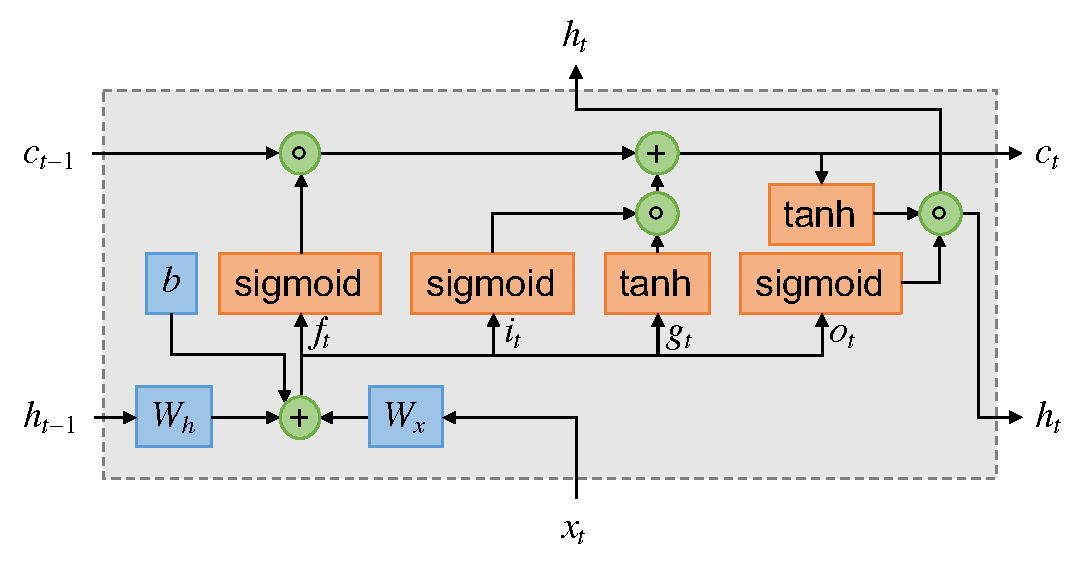
\includegraphics[width=\fig\textwidth]{3-04.pdf}
    \caption{Visulization for LSTM cell.}
    \label{fig:lstmcell}
\end{figure}

\paragraph{Multilayer RNN}
PolygonRNN uses multilayer RNN with ConvLSTM cells. The connection between two neighboring layers can be described as follows, which means that the cell input of this layer comes from the cell output of the previous layer.
\begin{equation}\label{eq:cellconnect}
	x_t^{(k)} = h_t^{(k-1)}, \forall k \in \{2,3,\ldots,n\},
\end{equation}
where $n$ is the number of RNN layers or ConvLSTM cells, $k$ in the superscript denotes the $k$-th layer. Recall that the initial cell input (i.e. the cell input of the first layer) at time step $t$ consists of the spatial information $f$ from CNN (including the masks of boundary and vertices), the two previous vertices $v_{t-1}$ and $v_{t-2}$, and starting vertex $v_0$, here it is formulated as follows.
\begin{equation}\label{eq:concat}
	x_t = x_t^{(1)} = v_{t-1} \oplus v_{t-2} \oplus v_0 \oplus f,
\end{equation}
where $\oplus$ denotes the concatenation operation in the dimension of image channel. Thus, the equation \ref{eq:vnext} can be written as follows.
\begin{equation}\label{eq:probcomp}
	y_t = p(v_t \mid v_{t-1}, v_{t-2}) = \text{softmax}(W_y\text{vec}(h_t^{(n)})),
\end{equation}
where $W_y$ denotes the weights of the final fully connected layer, $\text{vec}(\cdot)$ denotes the vectorization function for a matrix. Figure \ref{fig:rnnconvlstm} shows the entire structure of the RNN part and highlights the process at time step $t$, using the same notation as the equations \ref{eq:cellconnect}, \ref{eq:concat} and \ref{eq:probcomp}.

\begin{figure}[!h]
	\centering
	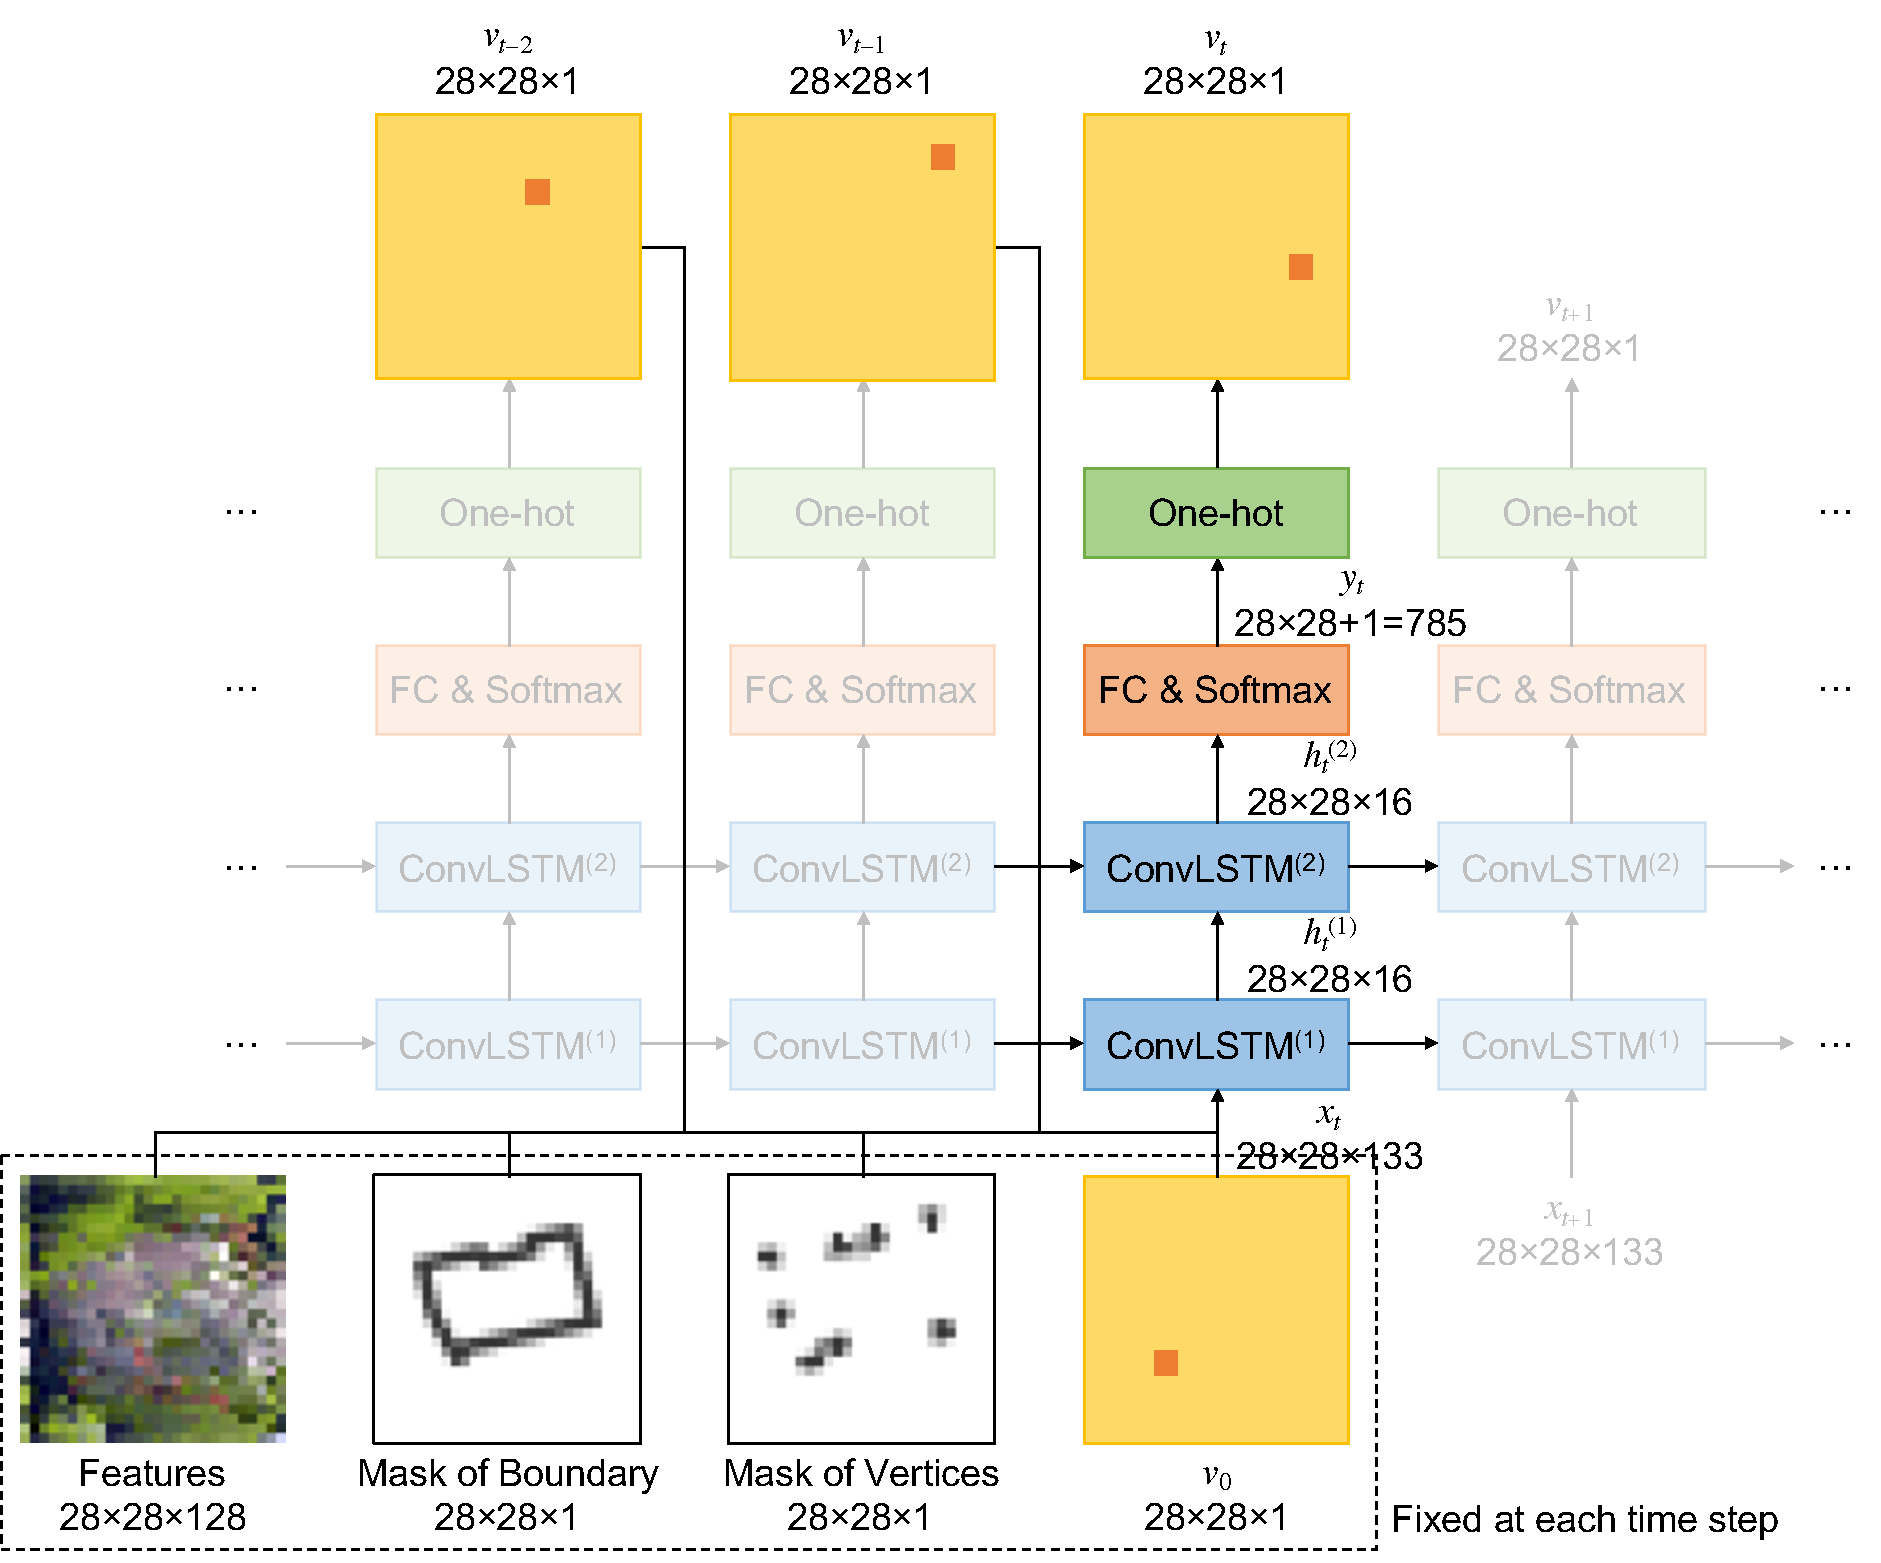
\includegraphics[width=\fig\textwidth]{3-05.pdf}
    \caption[Visualization for the time step of the RNN decoder]{Visualization for the time step of the RNN decoder. In this figure, the outputs of the end signal are omitted, and the configuration of the ConvLSTM cell is the same as what is used in the original PolygonRNN paper. Specifically, the paper sets the number of RNN layers to 2 and uses ConvLSTM cells with 3$\times$3 kernel size and 16 channels.}
    \label{fig:rnnconvlstm}
\end{figure}

Note that at each time step, the features, the masks of boundary and vertices as well as the one-hot encoding of starting vertex are fixed. Only $v_{t-1}$ and $v_{t-2}$ change over time.

\subsection{Loss Function}
The loss of PolygonRNN consists of two parts, loss of CNN and loss of RNN. The loss function of CNN part uses log loss, since the mask prediction is equivalent to binary classification for each pixel. We also notice that the non-boundary pixels or the non-vertex pixels occupy the majority, the loss function should be further weighted. As for the loss of RNN, the loss function used is cross-entropy loss, because the polygon prediction is equivalent to multiclass classification at every time step.

\section{Feature Pyramid Network}\label{modfpn}

FPN is the core model for object detection in this project. Object detection problem is exactly multiple bounding boxes regression problem, which finds out multiple RoIs within an image. Subsection \ref{sglbboxreg} first illustrates problem of single bounding box regression. Subsection \ref{ancpro} introduces some basic concepts related to anchor, and subsection \ref{mulbboxreg} further illustrates multiple bounding boxes regression. Finally, subsection \ref{bonefpn} looks into the backbone of FPN, presents how feature pyramid is generated and how FPN can tackle the multi-scale detection problem.

\subsection{Single Bounding Box Regression}\label{sglbboxreg}

Single bounding box regression can be used for such a scenario, where the target image has only one RoI. Generally, a bounding box can be uniquely determined by four parameters, either box center and box size, denoting $(x, y)$ and $(w, h)$ or the coordinates of the upper left and lower right corners of the box, denoting $(l, u)$ and $(r, d)$. They have following relationships.
\begin{equation}
	\left[\begin{array}{c}
		x\\y\\w\\h
	\end{array}\right]=\frac{1}{2}\left[\begin{array}{cccc}
		1 & 0 & 1 & 0 \\
		0 & 1 & 0 & 1 \\
		-2 & 0 & 2 & 0 \\
		0 & -2 & 0 & 2
	\end{array}\right]\left[\begin{array}{c}
		l\\u\\r\\d
	\end{array}\right],
\end{equation}
\begin{equation}
	\left[\begin{array}{c}
		l\\u\\r\\d
	\end{array}\right]=\frac{1}{2}\left[\begin{array}{cccc}
		2 & 0 & -1 & 0 \\
		0 & 2 & 0 & -1 \\
		2 & 0 & 1 & 0 \\
		0 & 2 & 0 & 1
	\end{array}\right]\left[\begin{array}{c}
		x\\y\\w\\h
	\end{array}\right].
\end{equation}
Therefore, we can regard the problem of finding out single bounding box of RoI as a parameter regression problem. With the image as input, any set of the four parameters, $(x, y, w, h)$ or $(l, u, r, d)$, can be selected as the target of the regression. Figure \ref{fig:sglbboxreg} shows the architecture of the network for the single bounding box regression, using box center and size as outputs.

\begin{figure}[!h]
	\centering
	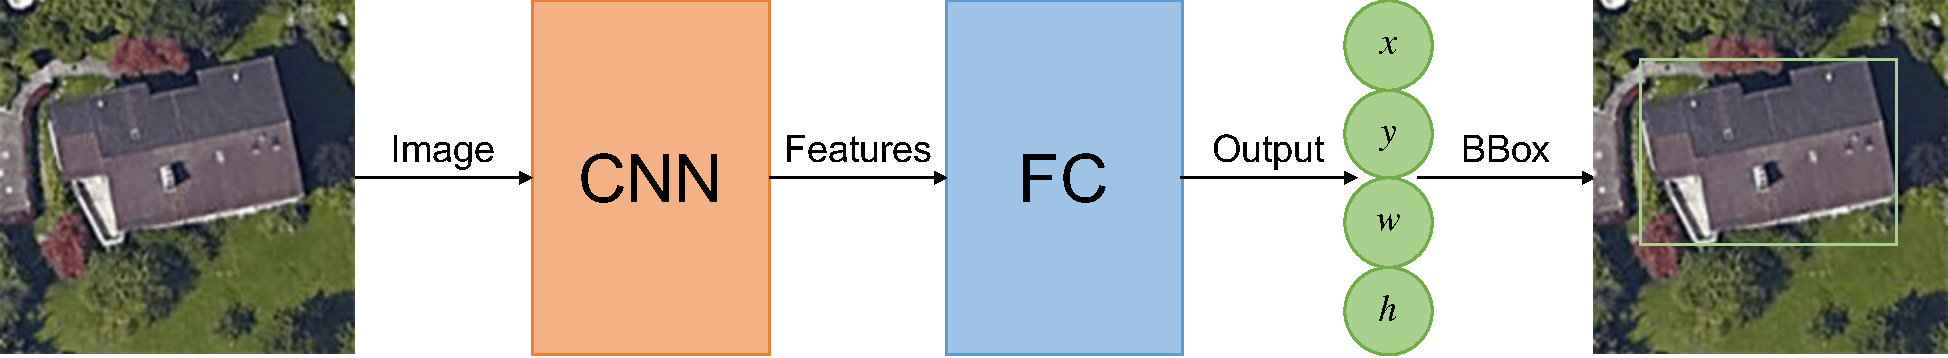
\includegraphics[width=\fig\textwidth]{3-06.pdf}
    \caption[Simplified structure of the network for single bounding box regression]{Simplified structure of the network for single bounding box regression. In this figure, the output of FC layer refers to the center and size of the bounding box.}
    \label{fig:sglbboxreg}
\end{figure}

In practice, usually the normalized parameters of box center and size rather than the coordinates of two corners are used as training targets. As for the normalization functions, see subsection \ref{mulbboxreg} for more details.

\subsection{Anchor and its Properties}\label{ancpro}
Anchor is a basic concept in multiple bounding boxes regression. The following paragraphs introduce the idea of anchor and its properties in detail.

\paragraph{Anchor}
An anchor refers to an artificially specified bounding box in the original image, regardless of the number of RoIs or where these RoIs locate. An arbitrary rectangular area in the image can be an anchor. For an image with width $w$ and height $h$, the total number of possible anchors $n$ can be calculated as
\begin{equation}\label{eq:numanchor}
	n = \frac{1}{4}w(w+1)h(h+1).
\end{equation}
Thus, even for a very small image patch with size 224$\times$224, $n$ is already very large, reaching 635.04 million. Figure \ref{fig:eganchor} illustrates some examples of anchors in an image with multiple RoIs.

\begin{figure}[!h]
	\centering
	\subbottom[]
		{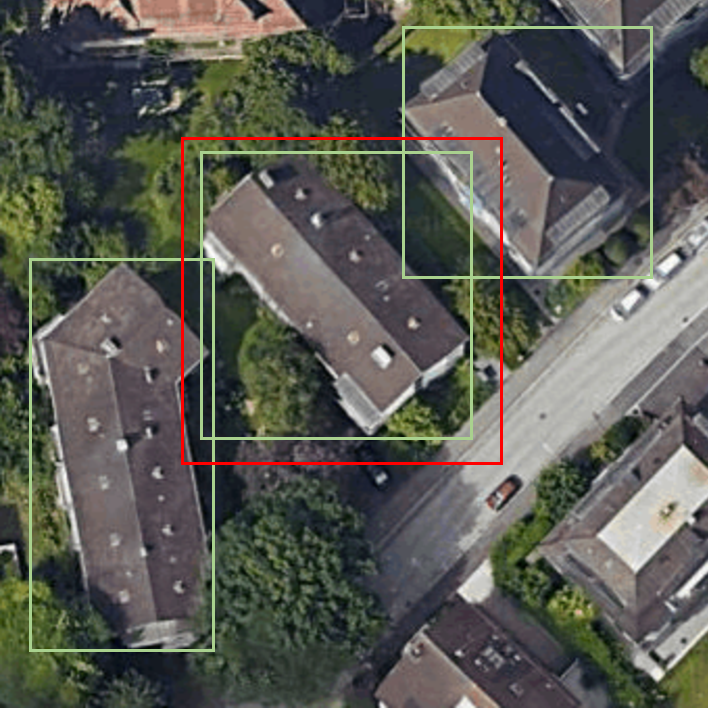
\includegraphics[width=\figfigfigfig\textwidth]{3-07-0.pdf}}
	\subbottom[]
		{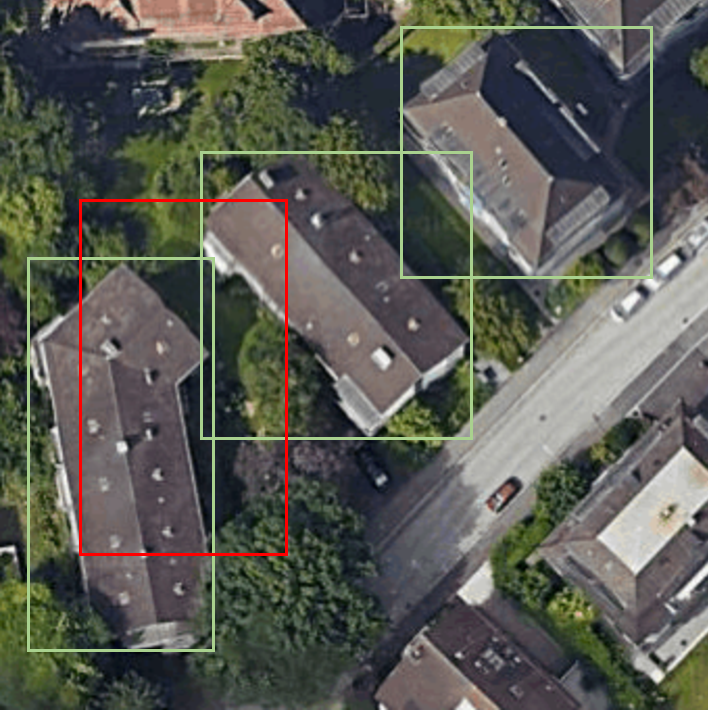
\includegraphics[width=\figfigfigfig\textwidth]{3-07-1.pdf}}
	\subbottom[]
		{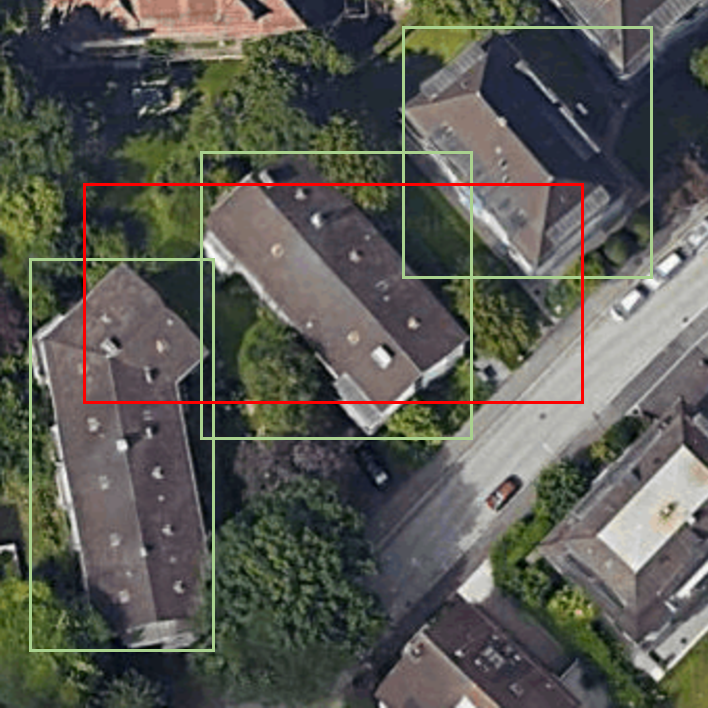
\includegraphics[width=\figfigfigfig\textwidth]{3-07-2.pdf}}
	\subbottom[]
		{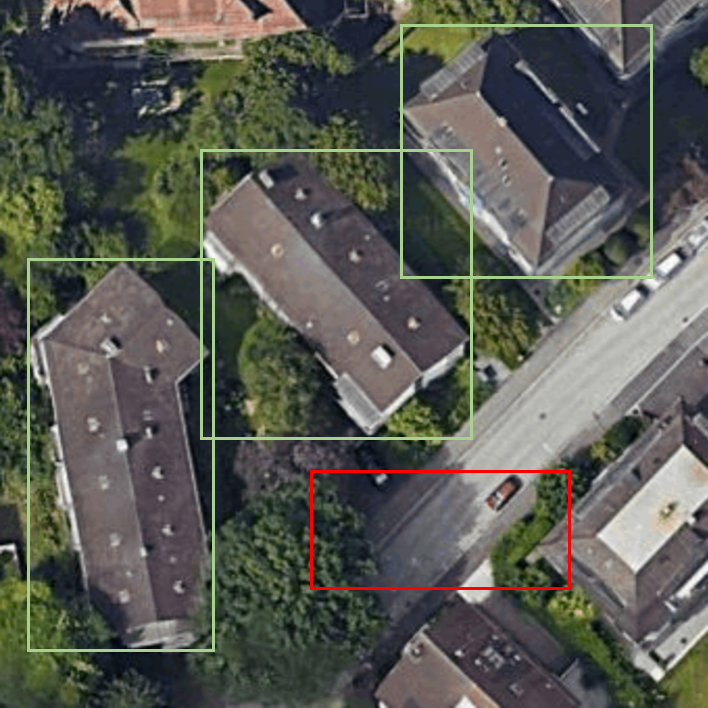
\includegraphics[width=\figfigfigfig\textwidth]{3-07-3.pdf}}
    \caption[Example anchors in image with multiple RoIs]{Example anchors in image  with multiple RoIs. (a)--(d) show four possible anchors in an image with  with multiple RoIs, with each showing one anchor. The red and light green rectangles refer to anchors and ground truth bounding boxes respectively.}
	\label{fig:eganchor}
\end{figure}

\paragraph{IoU Score}
Usually IoU (Intersection over Union) score is used to evaluate the similarity between an anchor and a ground truth bounding box. The following equation shows its computation.
\begin{equation}
	s = \frac{A \cap T}{A \cup T} \in [0, 1],
\end{equation}
where $s$ denotes the IoU score, $A$ and $T$ refer to the sets of pixels covered by the anchor and the ground truth bounding box respectively. $s = 1$ means that the anchor and the ground truth bounding box overlap perfectly. Figure \ref{fig:egiou} shows the coverage level under different IoU scores.

\begin{figure}[!h]
	\centering
	\subbottom[IoU = 0]
		{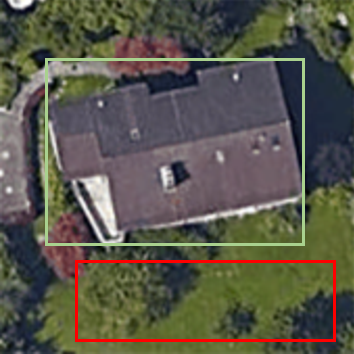
\includegraphics[width=\figfigfigfig\textwidth]{3-08-0.pdf}}
	\subbottom[IoU = 0.3]
		{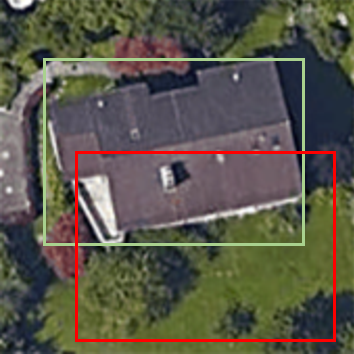
\includegraphics[width=\figfigfigfig\textwidth]{3-08-1.pdf}}
	\subbottom[IoU = 0.7]
		{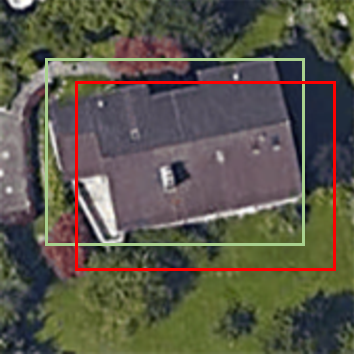
\includegraphics[width=\figfigfigfig\textwidth]{3-08-2.pdf}}
	\subbottom[IoU = 1]
		{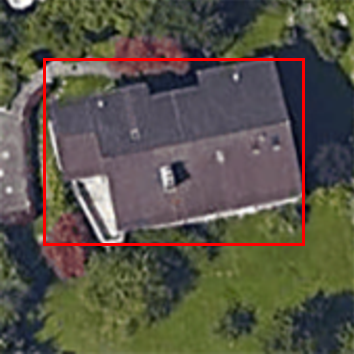
\includegraphics[width=\figfigfigfig\textwidth]{3-08-3.pdf}}
    \caption[Coverage level of anchor and ground truth bounding box under different IoU scores]{Coverage level of anchor and ground truth bounding box under different IoU scores.}
	\label{fig:egiou}
\end{figure}

\paragraph{Anchor Polarity}
Generally, there are several buildings in an aerial image, thus multiple RoIs exist. Based on the IoU scores of an anchor with these ground truth bounding boxes, we can make a judgment on the polarity of this anchor, which is defined as follows.
\begin{equation}
	d_i = \argmax_{j} \text{IoU}(a_i, g_j),
\end{equation}
\begin{equation}
	s_i = \text{IoU}(a_i, g_{d_i}),
\end{equation}
\begin{equation}
\begin{aligned}
	p_i = \begin{cases}
		1, & s_i > t_h, \\
		0, & t_l \leqslant s_i \leqslant t_h,\\
		-1, & s_i < t_l,
	\end{cases}
\end{aligned}
\end{equation}
where $a_i$ and $g_j$ denote the $i$-th anchor and $j$-th ground truth bounding box, $s_i$, $d_i$, and $p_i$ denote the highest IoU score that $a_i$ can get, the index of the `closest' ground truth box of $a_i$, and the polarity of $a_i$, $t_l$ and $t_h$ denote two threshold for the polarity judgment, and typically, $t_h = 0.7$, $t_l = 0.3$. An anchor is labeled as positive, natural or negative in case of $p_i = 1$, $p_i = 0$ or $p_i = -1$ respectively. Figure \ref{fig:eganchor} also shows anchors with different polarities.

\subsection{Multiple Bounding Boxes Regression}\label{mulbboxreg}
Multiple bounding boxes regression can be very different from the single one. Since the number of RoIs is unknown, if we still directly use the parameters regression as what we do in case of the single bounding box, then the number of nodes of the FC output layer will not be fixed. Besides, the RoIs in the image usually reflects the local information, usually we cannot directly use all global features obtained by CNN, either.

\paragraph{Anchor Assignment}
The basic idea for multiple bounding boxes regression is to regress them on positive anchors. Specifically, each RoI is regressed on the anchors which are assigned to it. There are two rules for the assignment: (1) each ground truth bounding box should have at least one anchor (either positive, natural or negative) assigned to it; (2) each positive anchor should be assigned to its `closest' ground truth bounding box. For those non-positive anchors that have assignments, we also treat them as positive anchors. For details of the matching algorithm, please refer to section \ref{app:assignanchor}.

\paragraph{Classification and Regression on Anchors}
As a matter of fact, the single bounding box regression can be regarded as regression on the anchor, which is exactly the whole image. Similar to this, we can simply increase the number of nodes in the FC output layer (see figure \ref{fig:sglbboxreg}) according to the number of anchors. Generally, each anchor requires 6 output nodes, 2 for binary classification and 4 for parameters regression. Specifically, 2 classification nodes output the logits, denoting $l_p$ and $l_n$, indicating how close the anchor is to an RoI. Thus the predicted probability of an anchor referring to an RoI $p^*$ can be described as
\begin{equation}
	p^* = \frac{e^{l_p}}{e^{l_p} + e^{l_n}}, 1 - p^* = \frac{e^{l_n}}{e^{l_p} + e^{l_n}}.
\end{equation}
The rest 4 regression nodes output the refined box information, for recovering the corresponding RoI. Suppose we have a fixed positive anchor, which is assigned to a ground truth bounding box. The refined (or normalized) box parameters are used for regression target, which can be described as follows.
\begin{equation}
	r_x = \frac{x_g - x_a}{w_a}, r_y = \frac{y_g - y_a}{h_a}, r_w = \log\frac{w_g}{w_a}, r_h = \log\frac{h_g}{h_a},
\end{equation}
where $(x_a, y_a, w_a, h_a)$ and $(x_g, y_g, w_g, h_g)$ denotes the four parameters of the anchor and the ground truth bounding box respectively, $(r_x, r_y, r_w, r_h)$ denotes the refined parameters for regression target. As for the recovery phase, we have
\begin{equation}
	x_g^* = x_a + r_x^*w_a, y_g^* = h_a + r_y^*h_a, w_g^* = w_ae^{r_w^*}, h_g^* = h_ae^{r_h^*},
\end{equation}
where $(r_x^*, r_y^*, r_w^*, r_h^*)$ and $(x_g^*, y_g^*, w_g^*, h_g^*)$ denote the predicted refinement parameters and the parameters of the final predicted bounding box respectively. The reason why the refined parameters are used for training, instead of original box, is that the former one eliminates the location information thus more reasonable.

\paragraph{Loss}
As for training, only positive and negative anchors are used, where classification uses both and regression only uses positive anchors. The loss used for classification is the log loss, described as follows.
\begin{equation}
	L_c = \mathbb{1}[p = 1]\log{\frac{1}{p^*}} + \mathbb{1}[p = -1]\log{\frac{1}{1-p^*}},
\end{equation}
where $L_c$ is the classification loss, $p$ is the polarity of the anchor, $p'$ is the predicted probability, $\mathbb{1}[\cdot]$ is the indicator function. The loss used for regression is the smooth $L_1$ loss, described as follows.
\begin{equation}
\begin{aligned}
	f(x) = \begin{cases}
		\dfrac{1}{2}x^2, & \lvert x \rvert < 1, \\
		\lvert x \rvert - \dfrac{1}{2}, & \lvert x \rvert \geqslant 1,
	\end{cases}
\end{aligned}
\end{equation}
\begin{figure}[!h]
	\centering
	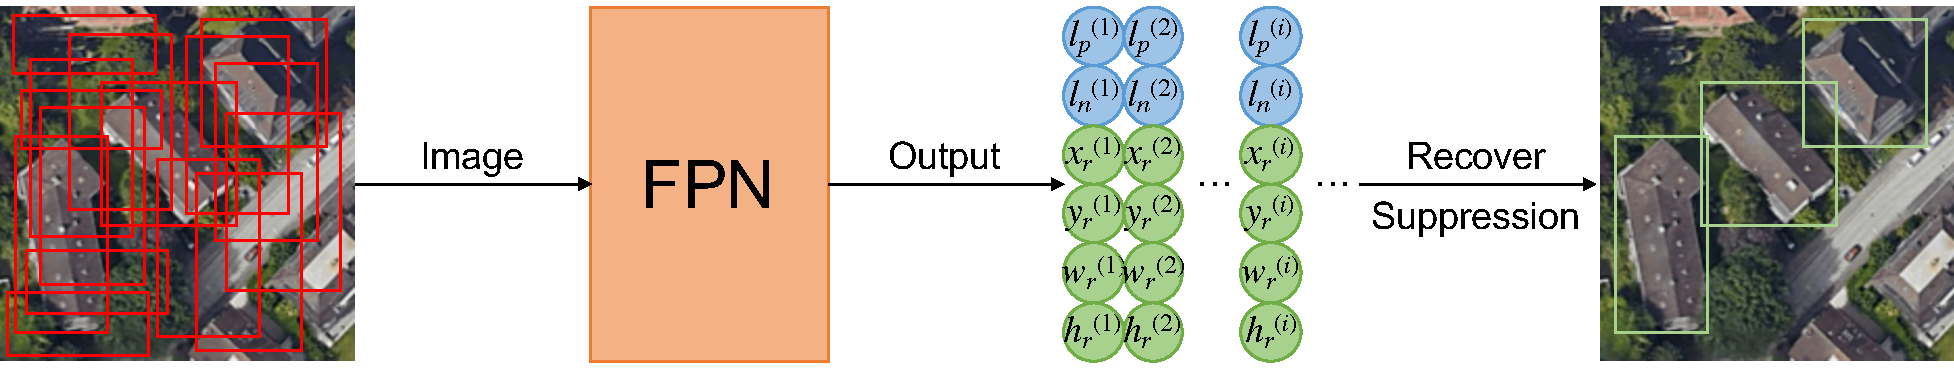
\includegraphics[width=\fig\textwidth]{3-09.pdf}
    \caption[Smooth $L_1$ loss function]{Smooth $L_1$ loss function.}
    \label{fig:l1loss}
\end{figure}
\begin{equation}
	L_r = f(x_g^* - x_g) + f(y_g^* - y_g) + f(w_g^* - w_g) + f(h_g^* - h_g),
\end{equation}
where $L_r$ is the regression loss. The total loss is defined as
\begin{equation}
	L = \sum_{i}^{} L_c^{(i)} + \lambda\sum_{i}^{}\mathbb{1}[p_i = 1]L_r^{(i)},
\end{equation}
where $\lambda$ is a self-defined parameter.

\subsection{Backbone and Feature Pyramid}\label{bonefpn}

\ref{eq:numanchor}
Suppose we have numbers of self-defined anchors. These anchors are evenly distributed in the image and have kinds of shapes. 
ResNet-101

Feature pyramids are a basic component in recognition systems for detecting objects at different scales. But recent deep learning object detectors have avoided pyramid rep- resentations, in part because they are compute and memory intensive. In this paper, we exploit the inherent multi-scale, pyramidal hierarchy of deep convolutional networks to con- struct feature pyramids with marginal extra cost. A top- down architecture with lateral connections is developed for building high-level semantic feature maps at all scales. This architecture, called a Feature Pyramid Network (FPN), shows significant improvement as a generic feature extrac- tor in several applications. Using FPN in a basic Faster R-CNN system, our method achieves state-of-the-art single- model results on the COCO detection benchmark without bells and whistles, surpassing all existing single-model en- tries including those from the COCO 2016 challenge win- ners. In addition, our method can run at 6 FPS on a GPU and thus is a practical and accurate solution to multi-scale object detection. Code will be made publicly available.


FPN uses a top-down architecture with lateral connections to build an in-network feature pyramid from a single-scale input. Faster R-CNN with an FPN back- bone extracts RoI features from different levels of the fea- ture pyramid according to their scale, but otherwise the rest of the approach is similar to vanilla ResNet. Using a ResNet-FPN backbone for feature extraction with Mask R- CNN gives excellent gains in both accuracy and speed. For further details on FPN, we refer readers to [27].

For the network head we closely follow architectures presented in previous work to which we add a fully con- volutional mask prediction branch. Specifically, we ex- tend the Faster R-CNN box heads from the ResNet [19] and FPN [27] papers. Details are shown in Figure 3. The head on the ResNet-C4 backbone includes the 5-th stage of ResNet (namely, the 9-layer ‘res5’ [19]), which is compute- intensive. For FPN, the backbone already includes res5 and thus allows for a more efficient head that uses fewer filters.
We note that our mask branches have a straightforward structure. More complex designs have the potential to im- prove performance but are not the focus of this work.



Dummy text.

\section{\modelnameshort}\label{modmer}

Dummy text.

\subsection{Two-step Model}

Dummy text.

\subsection{Hybrid Model}

Dummy text.

\subsection{Hybrid Model with RoI Align}




